\documentclass[11pt,a4paper]{article}
\usepackage[utf8]{inputenc}
\usepackage[english]{babel}
\usepackage{url}
\usepackage{csquotes}
\usepackage{graphicx}
\graphicspath{ {./images/} }

\usepackage{color}

\definecolor{pblue}{rgb}{0.13,0.13,1}
\definecolor{pgreen}{rgb}{0,0.5,0}
\definecolor{pred}{rgb}{0.9,0,0}
\definecolor{pgrey}{rgb}{0.46,0.45,0.48}

\usepackage{listings}
\lstset{language=Java,
  showspaces=false,
  showtabs=true,
  breaklines=true,
  showstringspaces=false,
  breakatwhitespace=true,
  commentstyle=\color{pgreen},
  keywordstyle=\color{pblue},
  stringstyle=\color{pred},
  basicstyle=\ttfamily,
  moredelim=[il][\textcolor{pgrey}]{$$},
  moredelim=[is][\textcolor{pgrey}]{\%\%}{\%\%}
}

\usepackage{biblatex}
\addbibresource{bibliography.bib}

\title{Garbage Collection Algorithm\\\small{Research Design}}

\author{Martijn Vegter - 500775388}
\date{October 18, 2020}

\begin{document}

\maketitle

\newpage
\section*{Abstract}
Garbage collection is the process of looking at heap memory, identifying unreferenced objects and the deleting of those. The memory used by an unreferenced object can thus be reclaimed. In Java, process of deallocating memory is handled automatically by the garbage collector.

The Parallel collector performs minor collections in parallel. It is supposed to maximize the throughput of the application. The mostly concurrent collectors perform most of their work concurrently, without `stopping the world'. This is supposed to keep pauses short and minimize the latency. The Java HotSpot VM offers two mostly concurrent collectors, the Concurrent Mark Sweep collector and the Garbage First collector.

The goal of this specific experiment is to find the most efficient garbage collector for a program that produces or handles a large quantity of short lived data. Even though the Concurrent Mark Sweep collector and the Garbage First collector are in the same category they had very different results.

The two best performing collectors, based on the the throughput and Stop-The-World times, are the Concurrent Mark Sweep collector and Parallel collector. From these two the Concurrent Mark Sweep collector is favored even though it has a lower throughput. The reason why the Concurrent Mark Sweep collector is favored is because of its heap usage.

Both during single- and multi-threaded workloads the heap is smaller and more stable as compared to the Parallel collector. For example during the single-threaded workloads both the used heap and the used Young is lower than the Parallel collector. During the multi-threaded workload the Parallel collectors showed a lot of instability especially towards the end.

While the experiment does provide insight in how different garbage collectors perform, the results are only representative for a very specific use case. That being said, even for the specific use case of high volume short lived data it is not completely representative as the system can and is expected to impact the results as the experiment ran on a laptop.

To account for any other applications or services requiring memory only 12.5\% (2 GB) of the available memory was allocated to the test program. Other hardware factors such as memory speed or CPU specifications limit the reproducibility of this research. Not to mention the software factors such as the Java SE Runtime Environment version, operating system and background processes utilizing the processor.

\newpage
\tableofcontents

\newpage
\section{Introduction}
Garbage collection is the process of looking at heap memory, identifying unused objects and the deleting of those. An in use object, or a referenced object, means that somewhere in the application a pointer to that object resides. An unused object, or unreferenced object, does not have an active pointer in the application. The memory used by an unreferenced object can thus be reclaimed. In Java, process of deallocating memory is handled automatically by the garbage collector. The basic process can be described as follows \cite{ORACLE_GC_BASICS}.

\subsection{Garbage Collecting}
\subsubsection*{Marking}
The first step in the process is called marking. This is where pieces of memory are identified as referenced or unreferenced. Referenced objects are shown in blue. Unreferenced objects are shown in gold. All objects are scanned in the marking phase to make this decision \cite{ORACLE_GC_BASICS}.

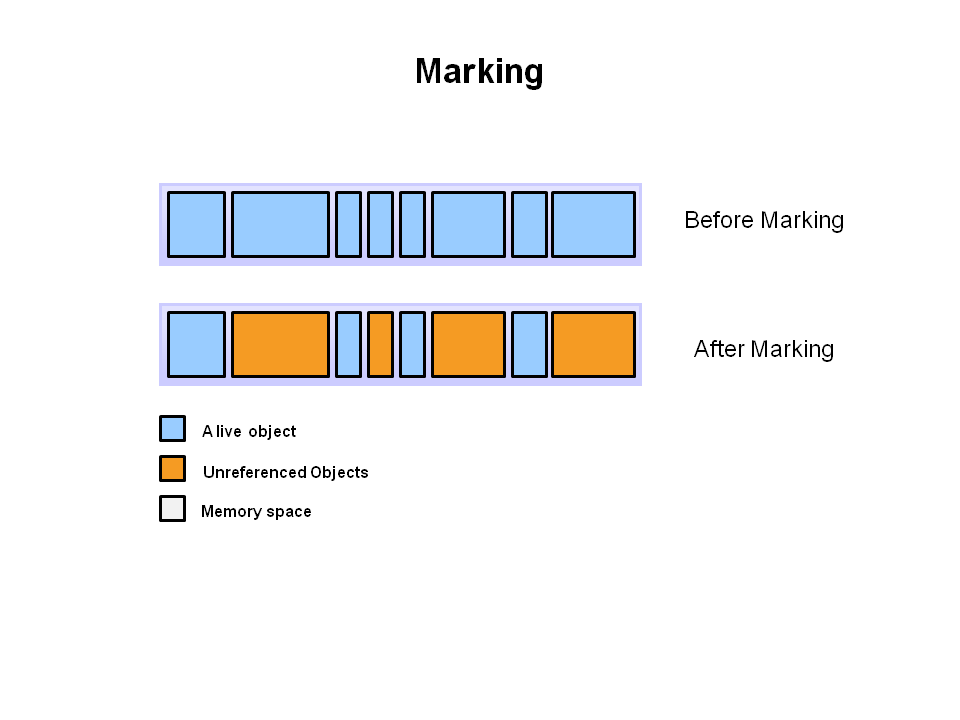
\includegraphics[width=0.5\textwidth]{Slide3.PNG}
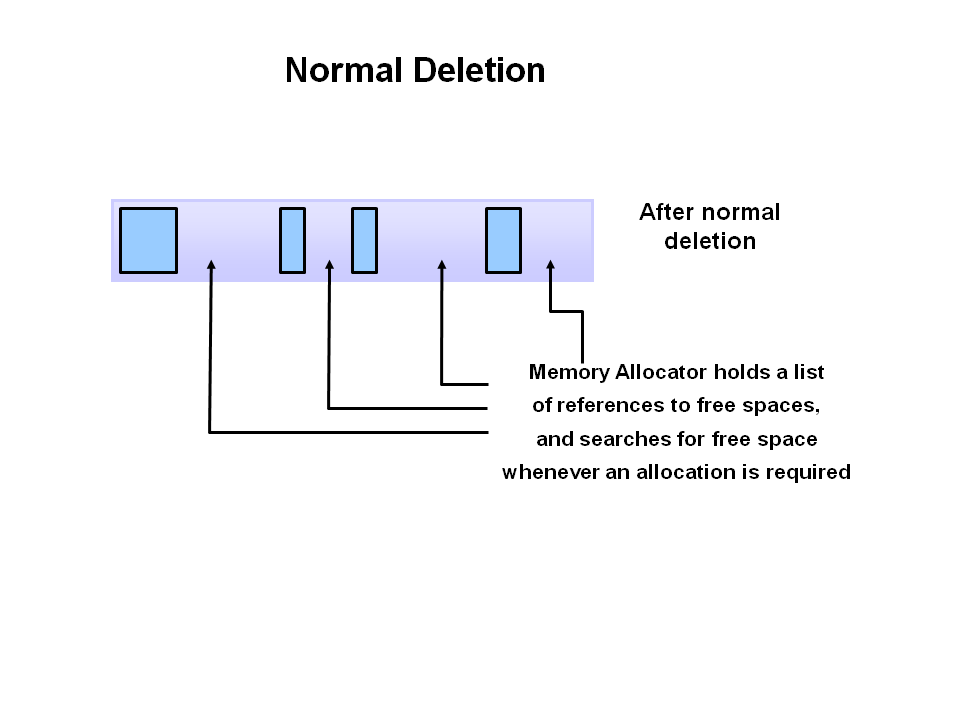
\includegraphics[width=0.5\textwidth]{Slide1b.PNG}

\subsubsection*{Normal Deletion}
Normal deletion removes unreferenced objects leaving referenced objects and pointers to free space. The memory allocator holds references to blocks of free space where new object can be allocated \cite{ORACLE_GC_BASICS}.

\subsection{JVM Generations}
The information learned from the object allocation behavior can be used to enhance the performance of the Java Virtual Machine (JVM). Therefore, the heap is broken up into smaller parts or so called generations. The heap parts are: Young Generation, Old or Tenured Generation, and Permanent Generation \cite{ORACLE_GENERATIONS}.

\begin{center}
    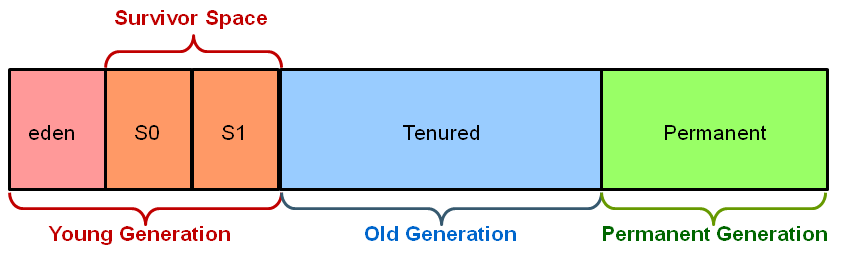
\includegraphics[width=0.75\textwidth]{Slide5.PNG}
\end{center}
\subsubsection*{Young Generation}
The Young Generation is where all new objects are allocated. When the young generation fills up, this causes a minor garbage collection. Minor collections can be optimized assuming a high object mortality rate. A young generation full of dead objects is collected very quickly. Some surviving objects are aged and eventually move to the old generation \cite{ORACLE_GC_BASICS}.

\subsubsection*{Old Generation}
The Old Generation is used to store long surviving objects. Typically, a threshold is set for young generation object and when that age is met, the object gets moved to the old generation. Eventually the old generation needs to be collected. This event is called a major garbage collection \cite{ORACLE_GC_BASICS}.

Major garbage collection are so called Stop-the-World events, all application threads are stopped until the operation completes. Often a major collection is much slower because it involves all live objects. The length of the Stop-the-World event for a major garbage collection is affected by the kind of garbage collector that is used for the old generation space \cite{ORACLE_GC_BASICS}.

\subsubsection*{Permanent Generation}
The Permanent generation contains metadata required by the JVM to describe the classes and methods used in the application. The permanent generation is populated by the JVM at runtime based on classes in use by the application. In addition, Java library classes and methods may be stored here. Classes may get collected (unloaded) if the JVM finds they are no longer needed and space may be needed for other classes. The permanent generation is included in a full garbage collection \cite{ORACLE_GC_BASICS}.
\newpage

\subsection{Garbage Collectors}
\subsubsection*{Concurrent Mark Sweep (CMS) Collector}
The Concurrent Mark Sweep (CMS) collector is designed for applications that prefer shorter garbage collection pauses and that can afford to share processor resources with the garbage collector while the application is running. Typically applications that have a relatively large set of long-lived data (a large old generation) and run on machines with two or more processors tend to benefit from the use of this collector \cite{ORACLE_CMS}.

\subsubsection*{G1 Garbage Collector}
The Garbage-First (G1) garbage collector is targeted for multiprocessor machines with a large amount of memory. It attempts to meet garbage collection pause-time goals with high probability while achieving high throughput with little need for configuration. G1 aims to provide the best balance between latency and throughput \cite{ORACLE_G1}.

\subsubsection*{Parallel  Collector}
The parallel collector (also referred to here as the throughput collector) is a generational collector similar to the serial collector. The primary difference between the serial and parallel collectors is that the parallel collector has multiple threads that are used to speed up garbage collection \cite{ORACLE_PARALLEL}.

\newpage
\section{Experimental setup}
The experiment is to figure out which of the three, before discussed, garbage collectors can most efficiently handle the large data volume produced by the test program. The term `efficiently' refers to the speed of the program. The experiment consists of two parts:
\begin{itemize}
    \item Gathering of the data
    \item Converting the data to information
\end{itemize}

\subsection{Gathering}
The source code of the mentioned classes and JVM configurations are available in the appendix.

The `ResearchDesign' class is responsible for creating an X number of threads which will execute the `MemoryHog' class. For the single-thread test this will result in two threads, the main program thread and a single thread running the `MemoryHog', the multi-threaded test has been set to create 5 threads.

The `MemoryHog' class creates 10.000 ArrayList instances containing Long's. Each ArrayList will contain 500.000 Long instances, note that the ArrayList will be initialized with the correct initial size. The size of a Long in Java 8 is 8 bytes. Each ArrayList will be roughly 4 megabytes. This repeated 10.000 times results in each 'MemoryHog' instance producing 40 gigabytes worth of Long's. In total 14.4 terabytes have been produced, by:
\begin{itemize}
    \item Each type of garbage collector; 4.8 terabytes each.
    \item Single- and multi-threaded each ran 20x; 240 gigabytes each.
    \item 1 thread from single- and 5 from multi-threaded; 40 gigabytes each.
\end{itemize}
Each run produced an output file from the garbage collector containing information regarding execution time, memory sizes and other detail information.

\subsection{Conversion}
The output files were uploaded to a self-hosted instance of GCPlot using the built-in REST API. GCPlot parses the log files and generates a report. Using the built-in REST API the report was extracted and converted into a CSV format to be able to import it to both Excel and IBM SPSS Statistics 26 for further analysis.

The graphs were generated by another tool called `GC Log Analyzer'. Further analysis was done by the built-in functionality of either Excel or SPSS.

\newpage
\section{Results}
The key metrics extracted from the reports are throughput, Stop-The-World, Promotion Rate and Allocation Rate. Throughput is the percentage of total time not spent in garbage collection. Stop-The-World refers to the amount of time the JVM stops the execution of the program to do a (full) garbage collection. Promotion rate is the amount of data moved from Young generation to Old generation per time unit. Allocation rate is the amount of memory allocated per time unit \cite{PLUMBR_BLOG}.

\subsection{Key performance indicators}
\subsubsection*{Single-threaded}
\begin{tabular}{lrr}
\hline
Name                    & Throughput          & Stop-The-World 99\%   \\ \hline
Concurrent Mark Sweep   & 92 \%               & 10.59 ms              \\
G1 Garbage              & 47 \%               & 190.78 ms             \\
Parallel                & 95 \%               & 7.89 ms               \\
&&\\
\hline
                        & Promotion Rate      & Allocation Rate       \\ \hline
                        & 6066.94 MB/Sec      & 0.14 MB/Sec           \\
                        & 639.89 MB/Sec       & 13453.22 MB/Sec       \\
                        & 5932.46 MB/Sec      & 1.77 MB/Sec
\end{tabular}

\vspace{10px}
Most notable is the difference in throughput between the Concurrent Mark Sweep and Parallel Garbage Collector compared to the G1 Garbage collector. The same applies for the promotion- and allocation rates. 

\subsubsection*{Multi-threaded}
\begin{tabular}{lrr}
\hline
Name                    & Throughput          & Stop-The-World 99\%   \\ \hline
Concurrent Mark Sweep   & 72 \%               & 27.94 ms              \\
G1 Garbage              & 31 \%               & 221.46 ms             \\
Parallel                & 79 \%               & 19.95 ms               \\
&&\\
\hline
                        & Promotion Rate      & Allocation Rate       \\ \hline
                        & 7517.29 MB/Sec      & 1.13 MB/Sec           \\
                        & 966.74 MB/Sec       & 809.21 MB/Sec       \\
                        & 8734.14 MB/Sec      & 36.26 MB/Sec
\end{tabular}

\vspace{10px}
The throughput has dropped a bit compared to the single-threaded performance while the promotion- and allocation rates have increased quite a bit. The 99 percentile Stop-The-World times have almost tripled for both the  Mark Sweep and Parallel Garbage Collector while the G1 Garbage Collector has only seen a small increase.

\newpage
\subsection{Heap Usage}
\begin{small}
    The Java heap is a repository for active objects, dead objects, and free memory.
    \begin{itemize}
        \item Blue - Free memory
        \item Blue - Used Heap
        \item Green - Used Tenured
        \item Purple - Used Young
    \end{itemize}
\end{small}

\subsubsection{Concurrent Mark Sweep (CMS) Collector}
\begin{tabular}{ c c }
    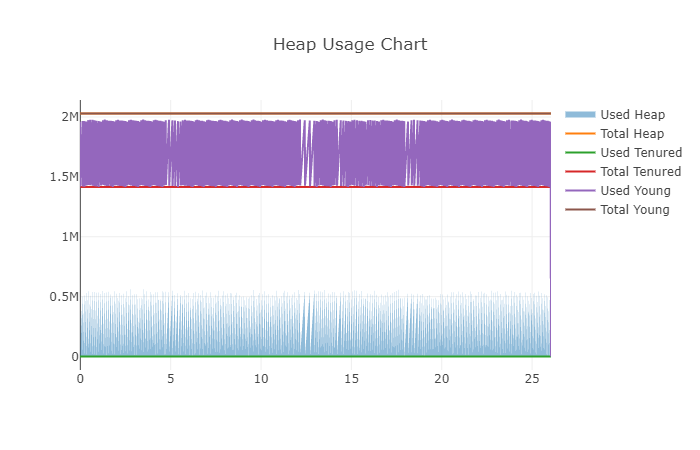
\includegraphics[width=0.5\linewidth]{heap_single_conc.png}         & 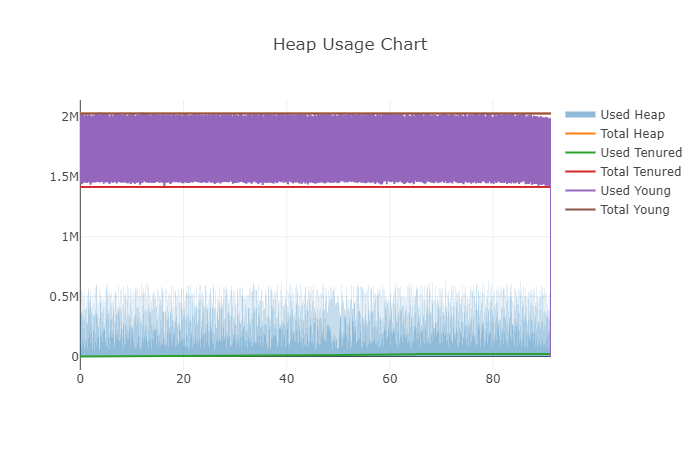
\includegraphics[width=0.5\linewidth]{heap_multi_conc.png} \\
    Single-threaded                                                     & Multi-threaded
\end{tabular}

\subsubsection{G1 Garbage Collector}
\begin{tabular}{ c c }
    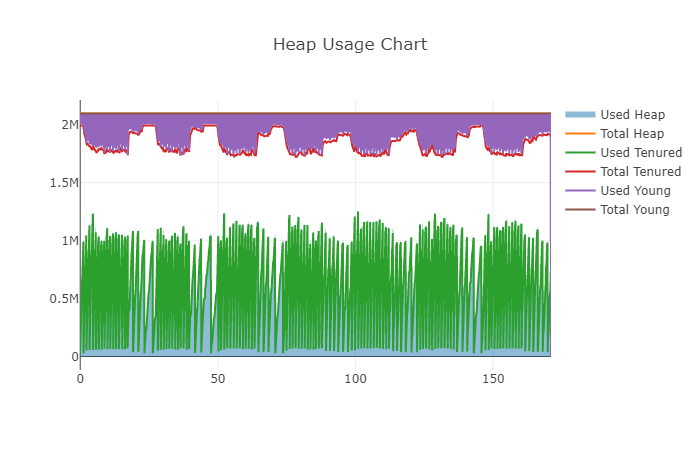
\includegraphics[width=0.5\linewidth]{heap_single_g1.png}           & 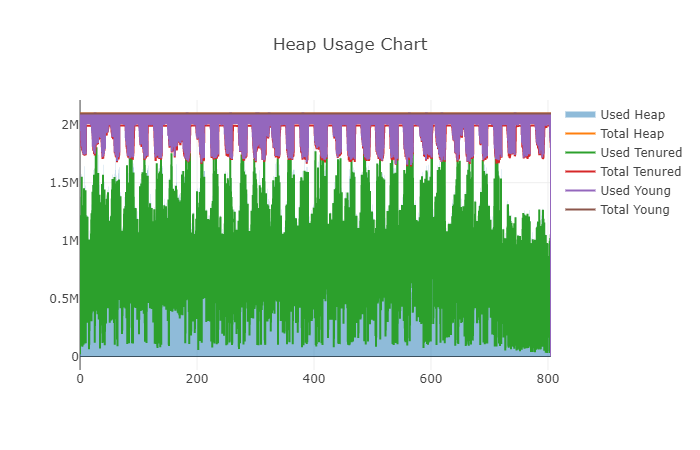
\includegraphics[width=0.5\linewidth]{heap_multi_g1.png} \\
    Single-threaded                                                     & Multi-threaded
\end{tabular}

\subsubsection{Parallel  Collector}
\begin{tabular}{ c c }
    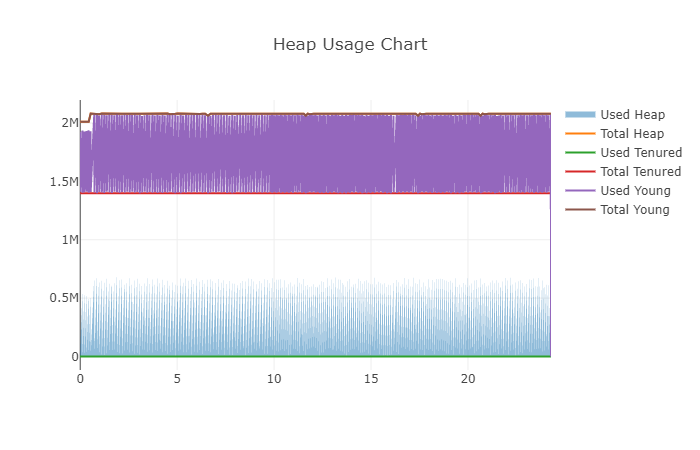
\includegraphics[width=0.5\linewidth]{heap_single_parallel.png}     & 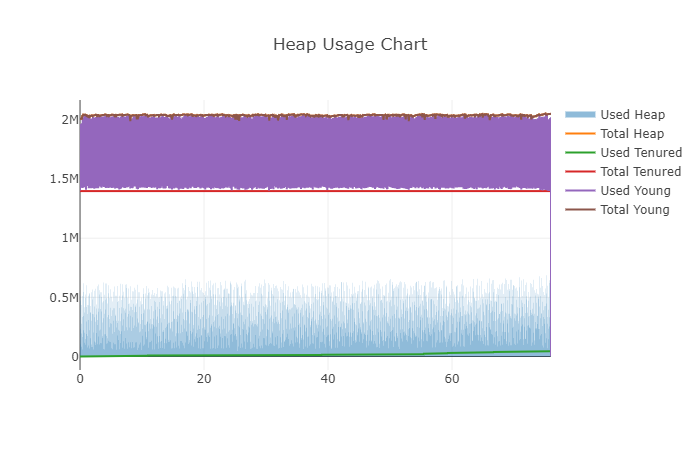
\includegraphics[width=0.5\linewidth]{heap_multi_parallel.png} \\
    Single-threaded                                                     & Multi-threaded
\end{tabular}

\newpage

\subsection{Correlations}
The individual correlations of single- and multi-thread are discusses together as both Correlations produced near the same results and equal significance. Comparing single- and multi-threaded against the other parameter is discusses separately.

\subsubsection{Correlations single- and multi-threaded}
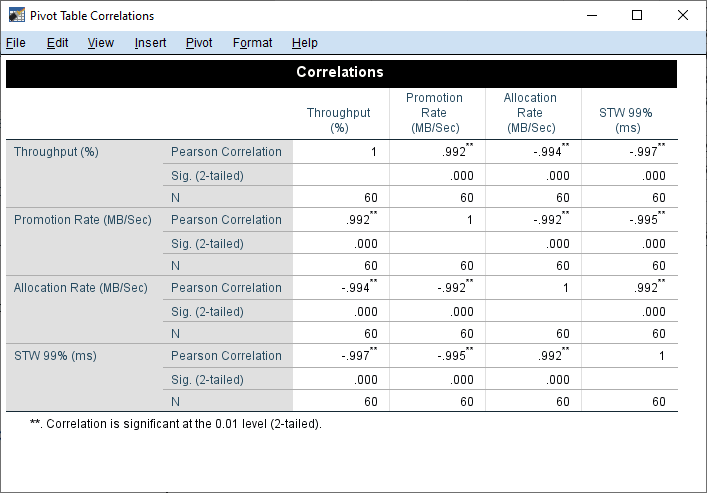
\includegraphics[width=\linewidth]{Correlations_single.png}
It is expected that a higher promotion rate results in a higher throughput as the test program is created to produce high volume, short lived data. From the Correlations table we can read that a, positive, significant correlation was found between promotion rate and throughput. Thus, a higher promotion rate results in a higher throughput.

It is expected that a higher allocation rate results in longer Stop-The-World time as the test program is created to produce high volume, short lived data. From the Correlations table we can read that a, positive, significant correlation was found between allocation rate and Stop-The-World times. Thus, a higher allocation rate results in a longer Stop-The-World times.

It is expected that a higher allocation rate results in a lower promotion rate as the results discussed before showed some kind of relation between the two Garbage Collector performance indicators. From the Correlations table we can read that a, negative, correlation was found. The reason for this is unclear but is recommend for further investigation.

\newpage
\subsubsection{Correlations single- versus multi-threaded}
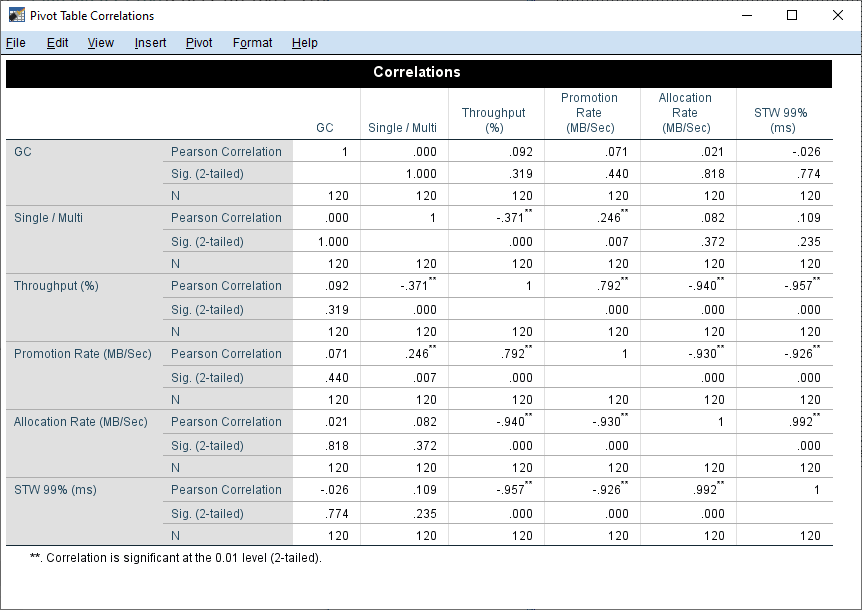
\includegraphics[width=\linewidth]{Correlations_single_multi.png}
It is expected that a higher throughput is achieved by the concurrent collectors as these types of garbage collectors have separate threads marking unused objects. From the table we can find that there is no significant correlation between two garbage collector types (low GC score is concurrent and high is parallel).

It is expected that the throughput of the multi-threaded runs is lower compared to the single threaded ones. From the table we can find a negative correlation between throughput and single- or multi-threaded run. The throughput is lower in multi-threaded runs.

It is expected that the Stop-The-World times increase as the total memory did not increase while the workload has increased. From the table we can find that there is no significant correlation between the single- or multi-threaded runs. The total workload did not affect the garbage collectors algorithms.

\newpage
\section{Conclusion}
The Parallel collector performs minor collections in parallel. It is supposed to maximize the throughput of the application. The mostly concurrent collectors perform most of their work concurrently, without `stopping the world'. This is supposed to keep pauses short and minimize the latency. The Java HotSpot VM offers two mostly concurrent collectors, the Concurrent Mark Sweep collector and the Garbage First collector \cite{ORACLE_AVAILABLE}.

The goal of this specific experiment is to find the most efficient garbage collector for a program that produces or handles a large quantity of short lived data. Even though the Concurrent Mark Sweep collector and the Garbage First collector are in the same category, namely the concurrent collectors. They had very different results.

The two best performing collectors, based on the the throughput and Stop-The-World times, are the Concurrent Mark Sweep collector and Parallel collector. From these two the Concurrent Mark Sweep collector is favored even though it has a lower throughput.

The reason why the Concurrent Mark Sweep collector is favored is because of its heap usage. Both during single- and multi-threaded workloads the heap is smaller and more stable as compared to the Parallel collector. For example during the single-threaded workloads both the used heap and the used Young is lower than the Parallel collector. During the multi-threaded workload the Parallel collectors showed a lot of instability especially towards the end.

The Tenured and Young spaces during the last phases of the program execution show a rising trend in their respective sizes. This same trend is visible for the Mark Sweep collector but the relative increase is a lot lower. Based on the heap usage the Concurrent Mark Sweep collector should be more scaleable than the Parallel Collector.

\newpage
\section{Discussion}
While the experiment does provide insight in how different garbage collectors perform, the results are only representative for a very specific use case. That being said, even for the specific use case of high volume short lived data it is not completely representative as the system can and is expected to impact the results as the experiment ran on a laptop.

To account for any other applications or services requiring memory only 12.5\% (2 GB) of the available memory was allocated to the test program. Other hardware factors such as memory speed or CPU specifications limit the reproducibility of this research. Not to mention the software factors such as the Java SE Runtime Environment version, operating system and background processes utilizing the processor.

In its purest sense, validity refers to how well a scientific test or piece of research actually measures what it sets out to, or how well it reflects the reality it claims to represent \cite{AQR_RELIABILITY}. In short, the validity of this paper is doubtable. The author has no prior experience with statistics nor the proper training or experience with tools required for doing the analysis.

\newpage
\printbibliography

\newpage
\section{Appendix}
\subsection{ResearchDesign.java}
\begin{lstlisting}[language=Java]
package com.martijnvegter;

import java.util.ArrayList;
import java.util.List;

class ResearchDesign {
  private static final int NUM_THREADS = 5;

  public static void main(String[] arg) {
    try {
      List<Thread> threads;
      
      threads = new ArrayList<>(NUM_THREADS);
      for (int i = 0; i < NUM_THREADS; i++) {
        Thread thread;
        
        thread = new Thread(new MemoryHog());
        threads.add(thread);
      }

      for (Thread thread : threads) {
        thread.start();
      }

      for (Thread thread : threads) {
        thread.join();
      }
    } catch (Exception e) {
      e.printStackTrace();
    }
  }
}
\end{lstlisting}

\newpage
\subsection{MemoryHog.java}
\begin{lstlisting}[language=Java]
package com.martijnvegter;

import java.util.ArrayList;
import java.util.List;

public class MemoryHog implements Runnable {
  private static final int NUM_LONGS = 500_000;
  private static final int NUM_LOOPS = 10_000;

  @Override
  public void run() {
    for (int j = 0; j < NUM_LOOPS; j++) {
      List<Long> longs;

      longs = new ArrayList<>(NUM_LONGS);
      for (int i = 0; i < NUM_LONGS; i++) {
        longs.add(new Long(i));
      }
    }
  }
}
\end{lstlisting}

\newpage
\subsection{generate.sh}
\begin{lstlisting}[language=bash]
#!/bin/bash
for gc in "ConcMarkSweep" "G1" "Parallel"
do
    for i in {1..20}
    do
        echo "java \
            -Xms2g \
            -Xmx2g \
            -verbose:gc \
            -XX:+PrintGCDetails \
            -XX:+PrintGCTimeStamps \
            -XX:+PrintGCDateStamps \
            -XX:+Use${gc}GC \
            -Xloggc:${gc}-${i}.log \
            com.martijnvegter.ResearchDesign" | sh
    done
done
\end{lstlisting}

\newpage
\subsection{Java HotSpot VM Options}
\subsubsection*{Concurrent Mark Sweep (CMS) Collector}
\begin{quote}
-XX:InitialHeapSize=2147483648

-XX:MaxHeapSize=2147483648

-XX:MaxNewSize=697933824

-XX:MaxTenuringThreshold=6

-XX:NewSize=697933824

-XX:OldPLABSize=16

-XX:OldSize=1395867648

-XX:+PrintGC

-XX:+PrintGCDateStamps

-XX:+PrintGCDetails

-XX:+PrintGCTimeStamps

-XX:+UseCompressedClassPointers

-XX:+UseCompressedOops

-XX:+UseConcMarkSweepGC

-XX:-UseLargePagesIndividualAllocation

-XX:+UseParNewGC
\end{quote}

\subsubsection*{G1 Garbage Collector}
\begin{quote}
-XX:InitialHeapSize=2147483648

-XX:MaxHeapSize=2147483648

-XX:+PrintGC

-XX:+PrintGCDateStamps

-XX:+PrintGCDetails

-XX:+PrintGCTimeStamps

-XX:+UseCompressedClassPointers

-XX:+UseCompressedOops

-XX:+UseG1GC

-XX:-UseLargePagesIndividualAllocation
\end{quote}

\newpage
\subsubsection*{Parallel  Collector}
\begin{quote}
-XX:InitialHeapSize=2147483648

-XX:MaxHeapSize=2147483648

-XX:+PrintGC

-XX:+PrintGCDateStamps

-XX:+PrintGCDetails

-XX:+PrintGCTimeStamps

-XX:+UseCompressedClassPointers

-XX:+UseCompressedOops

-XX:-UseLargePagesIndividualAllocation

-XX:+UseParallelGC
\end{quote}
\end{document}
